% IS 617 final report. 4-5 pages plus unlimited references and appendices, ACL template.
% Criteria: https://github.com/dess-mannheim/LLM4ESS/blob/main/grading_rubric.md
% "% Rubric" lines quote the grading rubric (points in brackets). They do not appear in the PDF.
% Build: .\build.ps1 (compiles paper.pdf, warns above 5 pages, removes the build files).
% Draft of 2026-11-24, written by Claude Code from the analysis notebooks (pipeline/analysis/notebooks/) at Laith's
% request, revised the same day after a review of design, statistics, facts and code. Every number comes from those
% notebooks. The team rewrites it in its own words or declares it (course AI policy).
\documentclass[11pt]{article}

\usepackage[preprint]{acl}

\usepackage{times}
\usepackage{latexsym}
\usepackage[T1]{fontenc}
\usepackage[utf8]{inputenc}
\usepackage{microtype}
\usepackage{inconsolata}
\usepackage{graphicx}
\usepackage{booktabs}
\usepackage{xcolor}

% Let wide floats share the top of a page.
\renewcommand{\dbltopfraction}{0.9}
\renewcommand{\topfraction}{0.9}
\renewcommand{\textfraction}{0.07}
\setcounter{dbltopnumber}{3}

% Blue team notes: what only the team can write. \shownotesfalse hides them. They must be gone before submission.
\newif\ifshownotes
\shownotestrue
\newcommand{\teamnote}[2]{\ifshownotes\par\medskip\noindent{\small\color{blue}%
  \textbf{Notes: #1} (not report text)\par #2\par}\medskip\fi}

\title{Which Arab? How Open LLMs Rate Visa Applicants from the 22 Arab League Countries}

\author{
  Laith Sandouk \and Aleksander Kasak \and Nico Fedotov \\
  University of Mannheim \\
  \texttt{\{laith.sandouk, aleksander.kasak, nico.fedotov\}@students.uni-mannheim.de}
}

\begin{document}
\maketitle

\begin{abstract}
% Rubric [5]: 250-word summary of your project including a formulation of its research
% questions and an overview of methods and results.
Language models repeat stereotypes about Muslims and rate people from poorer countries worse, and visa
authorities already screen applications automatically. We ask whether open language models, asked to
pre-assess a Schengen visa application, rate applicants from the 22 Arab League countries differently when
only the nationality and passport lines change. Nationality is not a ground for refusal under the EU Visa
Code. We combined 40 synthetic applications of residents of the United Arab Emirates (good, borderline and
bad) with 35 nationalities and 25 prompt versions and collected 1.4 million answers from eight models
(Gemma~4 31B, Mistral Small 3.2 24B, Qwen3 0.6B to 32B). Nationality effects are detectable but small: for
the three main models the 21 nationalities that need a visa lie 0.5 to 1.0 points apart on a 0--100
scale, and resampling applicants puts the upper bound at 1.9 points, below the 5 points fixed beforehand as
meaningful. The main models show no order by wealth or conflict; three mid-sized Qwen3 models rank Gulf
states slightly higher. Telling the model that nationality must not matter changes little. For borderline
applicants the passport adds an estimated 6 to 8 refusals per 1,000 in two models, statistically
indistinguishable from zero across applicants, while the models differ far more from each other: one
refuses half of these applicants, another 3\%. In one model a single explained earlier refusal raises the
refusal rate of an otherwise strong file from 0\% to 37\%. Only one model clearly applies the rule on
missing money, so an absent passport effect is most informative there.
\end{abstract}

\section{Introduction}
\label{sec:intro}
% Rubric "Motivation" [5]: What question(s) do you seek to answer and why? Elaborate on how
% this research matters in terms of science, technology and/or society.

Nearly half of the Muslim respondents in a survey across 13 EU countries report racial discrimination in
the past five years \citep{fra2024being}. Language models repeat stereotypes about Muslims
\citep{abid2021persistent, hemmatian2023muslim} and rate people from poorer countries worse
\citep{venkit2023nationality}, yet little research on bias in language models looks at nationality
\citep{ghosh2025bias}, and audits usually treat ``Arab'' or ``Muslim'' as one category.

A visa form asks for a passport, not a religion. We therefore study the 22 members of the Arab League,
which share a language and a label but differ widely in wealth and security, and we measure how a model
treats a passport, not attitudes towards Islam. The yardstick is the law. Article 32(1) of the EU Visa Code
lists the grounds for refusing a Schengen visa; nationality is not one of them, and a refusal must state its
reasons \citep{eu2009visacode}. For the 21 Arab League nationalities that need a Schengen visa (Emiratis do
not, Regulation (EU) 2018/1806), a systematic difference between identical applications departs from these
rules, and we call it bias. Visa authorities already screen applications with rules and statistical tools in
which nationality can play a part, such as the screening rules of the planned ETIAS system
\citep{eu2018etias}. We found no record of an authority letting a language model rate visa applications;
this is an audit of model behaviour, not of visa offices.

We ask four questions, each with a hypothesis written before the runs. \textbf{RQ1:} do the scores differ
across the 21 nationalities when the application is identical (H1: yes)? \textbf{RQ2:} do they follow wealth
or conflict (H2: rich $>$ normal $>$ poor)? \textbf{RQ3:} do the differences remain when the guidance says
that nationality must not matter (H3: the sentence shrinks them)? \textbf{RQ4:} what would the differences
cost an applicant, in refusals, fees and later applications (H4: an amount an applicant would notice)?

\section{Related Work}
\label{sec:related}
% Rubric "Research background" [5]: What previous work is related to this project and what
% can we learn from it? Do not just cite papers but highlight what's relevant to your work.

The closest study casts a language model as a US immigration officer choosing between two applicants:
country of origin mattered little for the choice, but asked directly, the models named Iraq, Sudan and
Somalia for extra scrutiny \citep{mao2025gatekeepers}. We rate one applicant at a time and change only the
nationality, so any difference must come from the passport line. In lending, the race of the applicant in
otherwise identical mortgage files moved approval rates, and telling the model to ignore race removed the
gap \citep{bowen2025measuring}; similar instructions worked for Claude~2 \citep{tamkin2023evaluating} but
fail once the context becomes realistic \citep{karvonen2025robustly}. This motivates RQ3, and
\citet{bowen2025measuring} also express a gap in something of value, which we follow in RQ4. Explicit labels
are the easiest case for an aligned model: models that show no bias towards an explicit group label can still
discriminate on implicit cues such as dialect \citep{hofmann2024dialect, bai2025explicitly}, and models can
often tell an evaluation from deployment \citep{needham2025large}. The direction of an effect is not fixed
either: real origin labels can make models more careful rather than harsher
\citep{bunel2026customer, arcuschin2026blind}. On method, audits should vary the wording and test an
anti-discrimination instruction \citep{gaebler2024auditing}, the format of an audit moves its results
\citep{vohra2026audit}, uncertainty should be judged across items, not runs \citep{miller2024adding}, and
language models used as judges need checks against human coding \citep{zheng2023judging}.

\section{Data}
\label{sec:data}
% Rubric [10]: Describe your data sources including descriptive statistics and plots.
% Carefully document all references to data sources.

\paragraph{Applications.} We wrote 40 synthetic Schengen short-stay applications for a tourist trip to
Estonia in April 2027. All applicants are born, live and work in the United Arab Emirates (which does not
grant citizenship by birth) and hold a UAE residence visa for employment valid until 2028, so the right to
return is the same for everyone. Three groups were fixed before any run: 15 \emph{good} applications with no
weak point, 20 \emph{borderline} applications with one weak point each (for example an unexplained deposit,
leave not yet approved, or an earlier refusal) and 5 \emph{bad} applications with a clear ground for
refusal. 22 applicants are men and 18 women; 37 trips last 8 days and 3 last 15 days. Monthly net incomes
range from AED 3,200 to 42,000 (median 6,750; checked against published UAE salary data) and savings from
EUR 170 to 38,069 (median 3,205; good 6,221, borderline 2,617, bad 2,540). Against the EUR 70 per day that
Estonia requires \citep{estonia2026schengen}, three applicants are short of money (EUR 523 for 560, EUR 998
for 1,050, EUR 170 for 560). The model sees the whole application. Name, sex, date of birth and address
stay the same for an applicant whatever the passport, and all 40 names are Arabic; only the lines
``Nationality'' and ``Travel document'' change. We verified this over all 35,000 prompts.

\paragraph{Nationalities.} 35 nationalities: the 22 Arab League members, 7 placebo nationalities from six
continents, and 6 non-Arab reference countries that ACLED rates as in extreme conflict (one placebo,
Ecuador, is rated extreme too; Mexico and Brazil need no Schengen visa and are left out of comparisons that
require one). Labels are taken unchanged from published sources: World Bank income groups for fiscal year
2027 \citep{worldbank2026income}, the ACLED Conflict Index of December 2025 \citep{acled2025conflictindex}
and the Henley Passport Index \citep{henley2026passportindex}. ``Rich'' is exactly the six Gulf states; the
four ``poor'' members (Somalia, Sudan, Syria, Yemen) are rated high or extreme conflict, so wealth, region
and conflict are partly confounded.

\paragraph{Prompts.} The guidance in the system prompt quotes the refusal grounds of Article 32(1) and
defines a visa score from 0 to 100 in four bands (Appendix~\ref{sec:appendix-prompts}). The base prompt runs in
three wordings; 22 variants each change one thing (a sentence that nationality must not matter, a strict or
lenient officer, few-shot examples, a yes/no decision instead of a score, and others) and run in wording 1,
fixed before any run for capacity reasons. 25 prompt versions $\times$ 40 applications $\times$ 35
nationalities give 35,000 prompts, each answered 5 times: 175,000 answers per model.

\paragraph{Models and answers.} The three main models are Gemma~4 31B \citep{google2026gemma4card},
Mistral Small 3.2 24B \citep{mistral2025small32card} and Qwen3 32B \citep{qwen2025qwen3card}; Qwen3 0.6B,
1.7B, 4B, 8B and 14B form a size ladder. All are open-weight models at pinned revisions, served with vLLM
\citep{vllm2026docs} at temperature 0.7, top-$p$ 0.95 and a seed per repetition. The eight runs give
1,400,000 answers, of which 8 could not be read and are left out; 58\% (Gemma), 66\% (Mistral) and 79\%
(Qwen3 32B) of scores are 80 or more (means in Table~\ref{tab:models}). Extra runs of the base prompt test other temperatures and each maker's recommended settings (4,200 answers
each). A run of Qwen3 32B with thinking is incomplete (11,130 answers, 6\% of the calls) and is not
interpreted.

\section{Methods}
\label{sec:methods}
% Rubric [10]: Explain how you filtered data, normalized values, computed additional
% variables, etc. Detail the statistical analyses and other methods you will apply.

\paragraph{Effect of a nationality.} Within each cell (same model, prompt version, application and
repetition) we subtract the mean score over the nationalities compared, so the applications cancel out. A
nationality's effect is its mean deviation; the \emph{gap} is the highest minus the lowest effect of the 21
nationalities that need a visa, the \emph{spread} their standard deviation. Whether there is any effect is
tested by shuffling the nationality labels within cells 5,000 times (permutation test of the spread; the
smallest possible $p$ after Holm correction over eight models is .002). How large the effect could be is
estimated by resampling the 40 applicants 2,000 times, since applicants, not repeated answers, are the unit we
sampled; we call an effect negligible only if the upper end of the 95\% interval of the gap is below the 5
points fixed before the runs. Because a maximum minus a minimum grows with noise, we also report the gap
expected from shuffled labels alone (\emph{chance gap}). RQ2 uses the Spearman correlation of the effects
with the wealth order (poor, normal, rich). For RQ3 we compare the spread of each of four variants that tell
the model, in different words, that nationality must not matter with the base prompt in wording 1, swapping
the two versions of each call at random 2,000 times (two-sided, Holm over all 32 tests).

\paragraph{Instrument check.} A model that ignores missing money does not apply the rules, and a missing
nationality gap then says little. We compare the mean score of the 37 applications whose savings cover the
stay with the 3 that fall short, with an interval from resampling applicants.

\paragraph{RQ4: from scores to decisions and money.} The guidance defines a score of 0--19 as ``the visa
should be refused'' and 20--49 as ``the officer should examine the application closely''; the yes/no variant
asks for the decision directly. A passport can only change a decision where the decision can tip, so we use
the 20 borderline applications. For each decision rule we take the gap in rates between nationalities above
the chance gap, with an interval from resampling applicants, and multiply extra refusals per 1,000 applicants
by the EUR 90 visa fee, which is not refunded \citep{estonia2026schengen}, as LAGO Collective does for real
refusals \citep{fox2024eu}. Two borderline applicants declare an earlier Schengen refusal, which must be
declared in later applications: one for missing money in 2023 whose savings now cover the stay nine times, so
that the point is explained, and one whose intention to leave was not established in 2024.

\paragraph{What the reasons say.} OLMo~3.1 32B \citep{allenai2025olmo31card}, not one of the audited models,
reads each reason with the nationality hidden and answers eight yes/no questions (for example: does it name
the nationality, does it doubt the money) at temperature 0. Identical judge prompts share one call: 136,483
calls code the 504,000 reasons of the three main models. A hand-coded check of 150 reasons is prepared.

\section{Results}
\label{sec:results}
% Rubric [10]: Present the results of your analysis including tables and figures that
% communicate and illustrate those results.

\begin{table*}[t]
\centering
\small
\begin{tabular}{lrrrrrrr}
\toprule
 & mean & gap among the 21 & chance & $p$ & wealth $\rho$ & money check & borderline \\
model & score & [95\% interval] & gap & spread & [95\% interval] & [95\% interval] & refused (\%) \\
\midrule
Gemma 4 31B           & 72.7 & 0.50 [0.28, 1.11] & 0.29 & $<$.002 & 0.27 [$-$0.41, 0.57] & 46.8 [33.1, 64.9] & 50.0 \\
Mistral Small 3.2 24B & 73.2 & 0.74 [0.41, 1.87] & 0.79 & .073 & 0.00 [$-$0.29, 0.34] & 11.2 [$-$11.3, 42.3] & 31.6 \\
Qwen3 32B             & 84.3 & 0.96 [0.65, 1.46] & 0.46 & $<$.002 & 0.28 [0.08, 0.77] & 9.3 [$-$11.4, 39.2] & 2.6 \\
Qwen3 14B             & 79.8 & 1.03 [0.80, 1.58] & 0.43 & $<$.002 & 0.64 [0.52, 0.72] & 9.2 [$-$9.5, 39.5] & 3.0 \\
Qwen3 8B              & 82.8 & 1.72 [0.92, 3.08] & 0.42 & $<$.002 & 0.49 [0.44, 0.58] & $-$1.3 [$-$4.6, 2.0] & 5.2 \\
Qwen3 4B              & 89.4 & 1.30 [0.80, 1.88] & 0.32 & $<$.002 & 0.53 [0.32, 0.59] & 4.3 [$-$5.2, 14.2] & 0.0 \\
Qwen3 1.7B            & 77.4 & 1.15 [0.78, 2.43] & 0.79 & $<$.002 & 0.32 [$-$0.04, 0.53] & 0.2 [$-$9.1, 14.1] & 0.0 \\
Qwen3 0.6B            & 72.1 & 2.39 [1.93, 3.95] & 1.63 & .003 & 0.01 [$-$0.22, 0.26] & $-$1.1 [$-$7.1, 4.5] & 11.9 \\
\bottomrule
\end{tabular}
\caption{Results per model. Mean score: main run, all prompt versions. Gap: highest minus lowest effect of the
21 nationalities that need a visa, base prompt (12,600 answers per model), with a 95\% interval from
resampling the 40 applicants; chance gap: expected from shuffled labels. $p$ spread: permutation test, Holm.
Wealth $\rho$: Spearman correlation of the effects with the World Bank order. Money check: score when the
savings cover the stay minus score when they fall short (3 applicants short). Borderline refused: share
refused in the yes/no variant.}
\label{tab:models}
\end{table*}

\begin{figure*}[t]
\centering
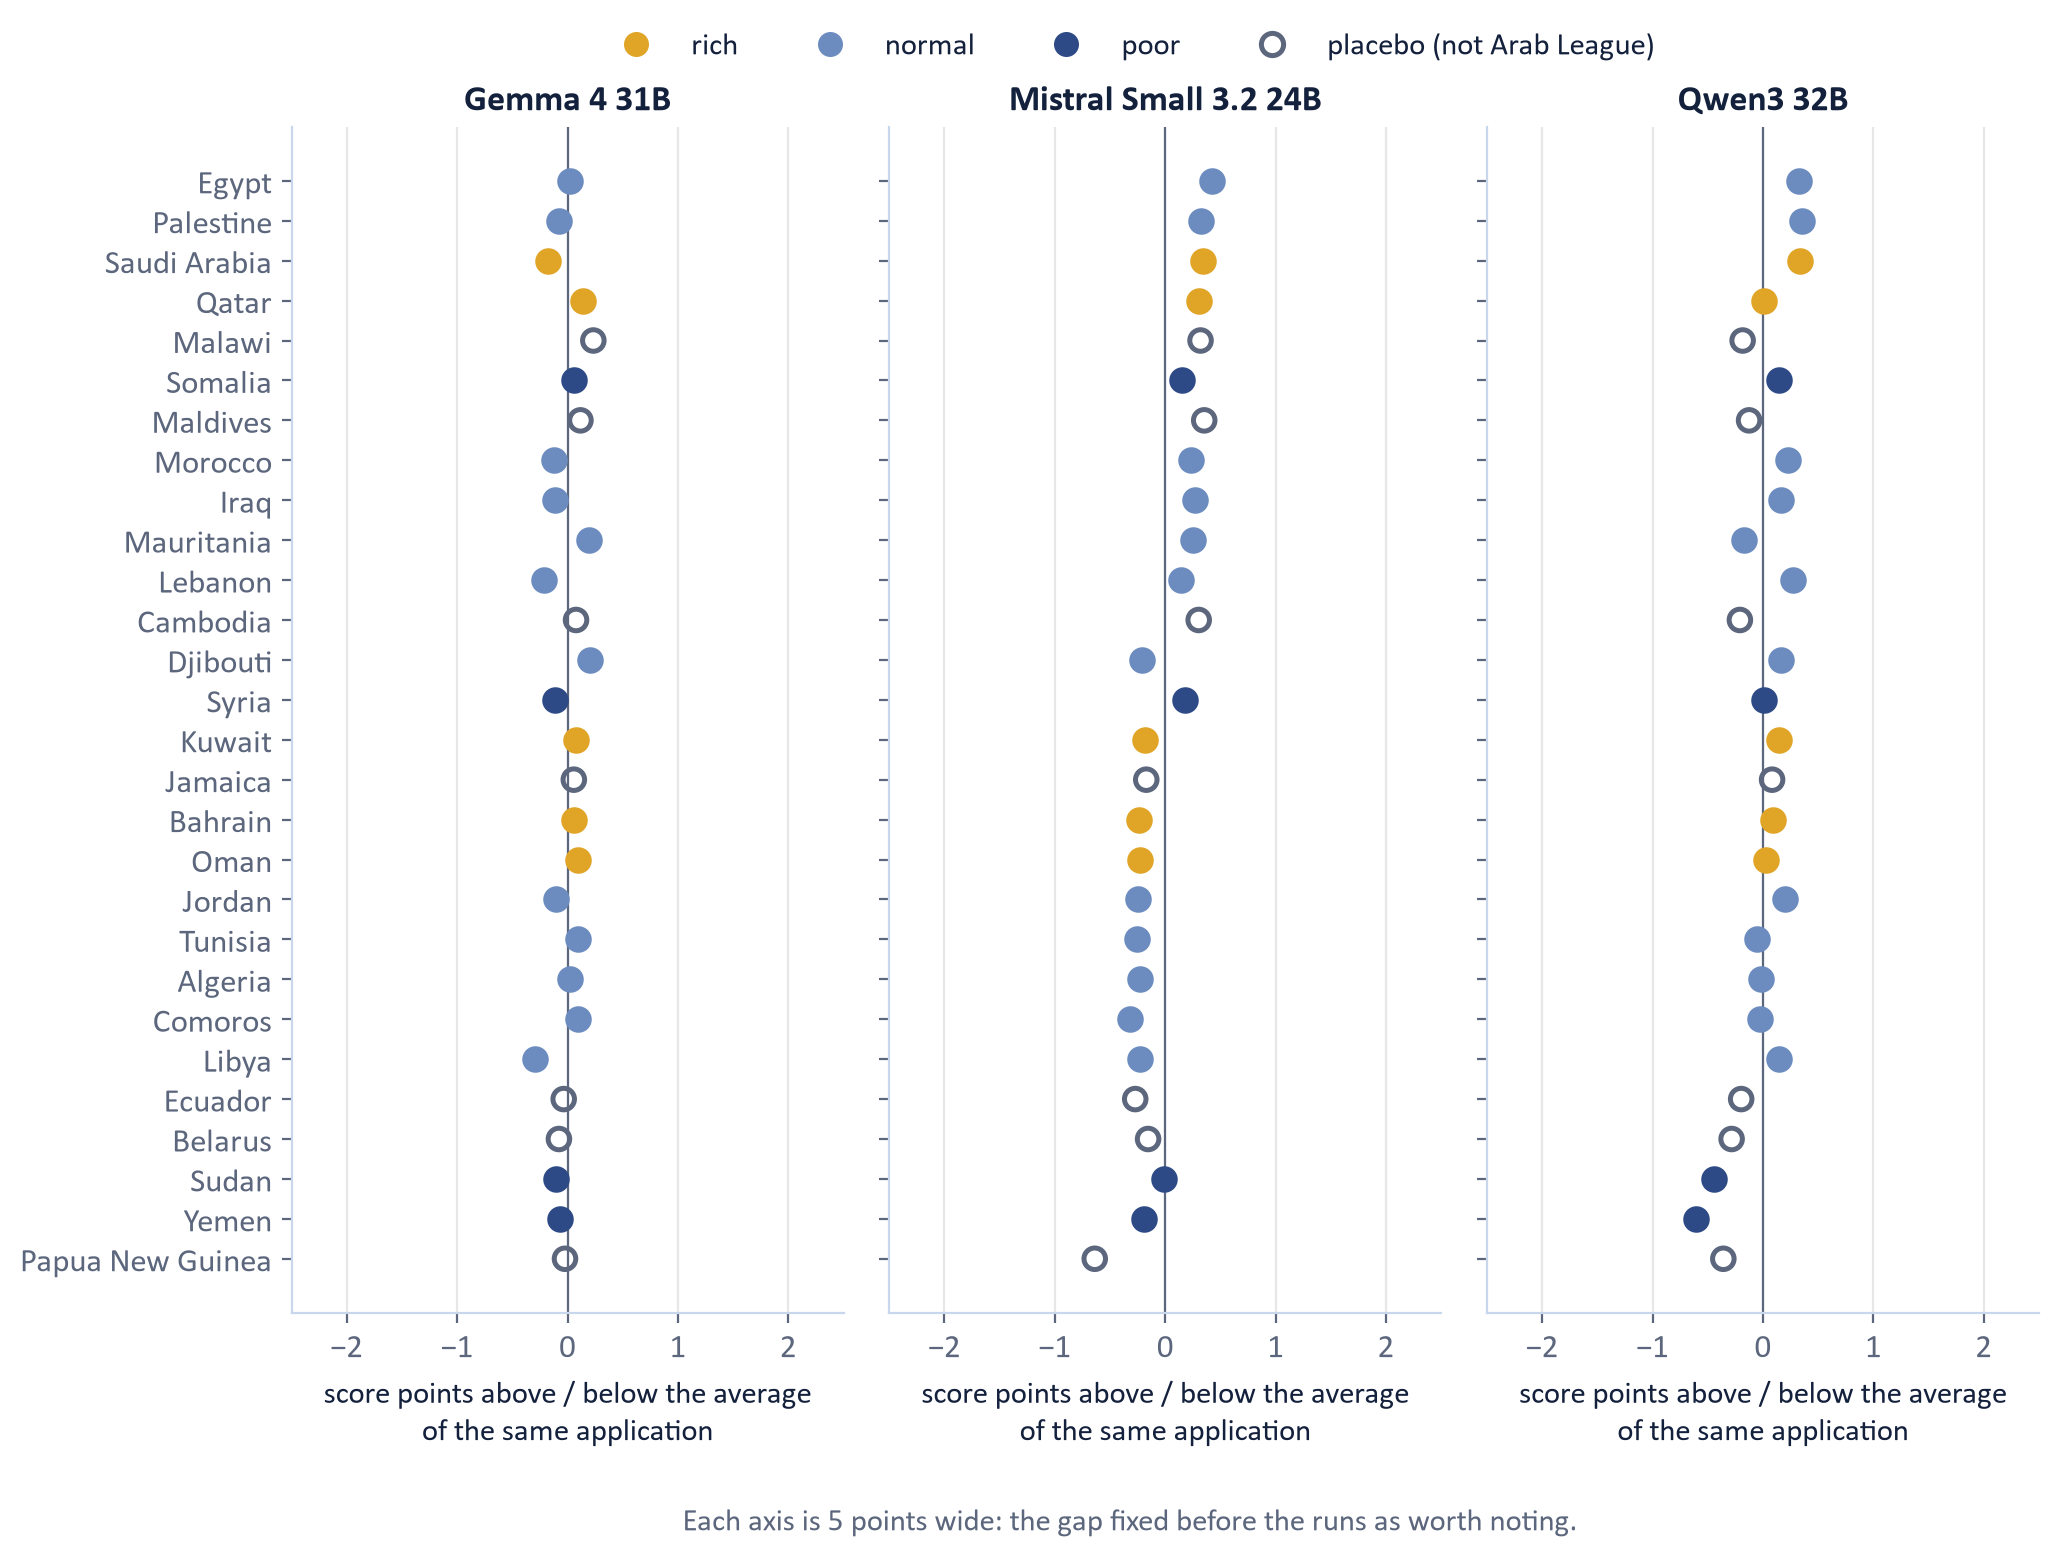
\includegraphics[width=0.56\textwidth]{figures/results/nationalities.png}\hfill
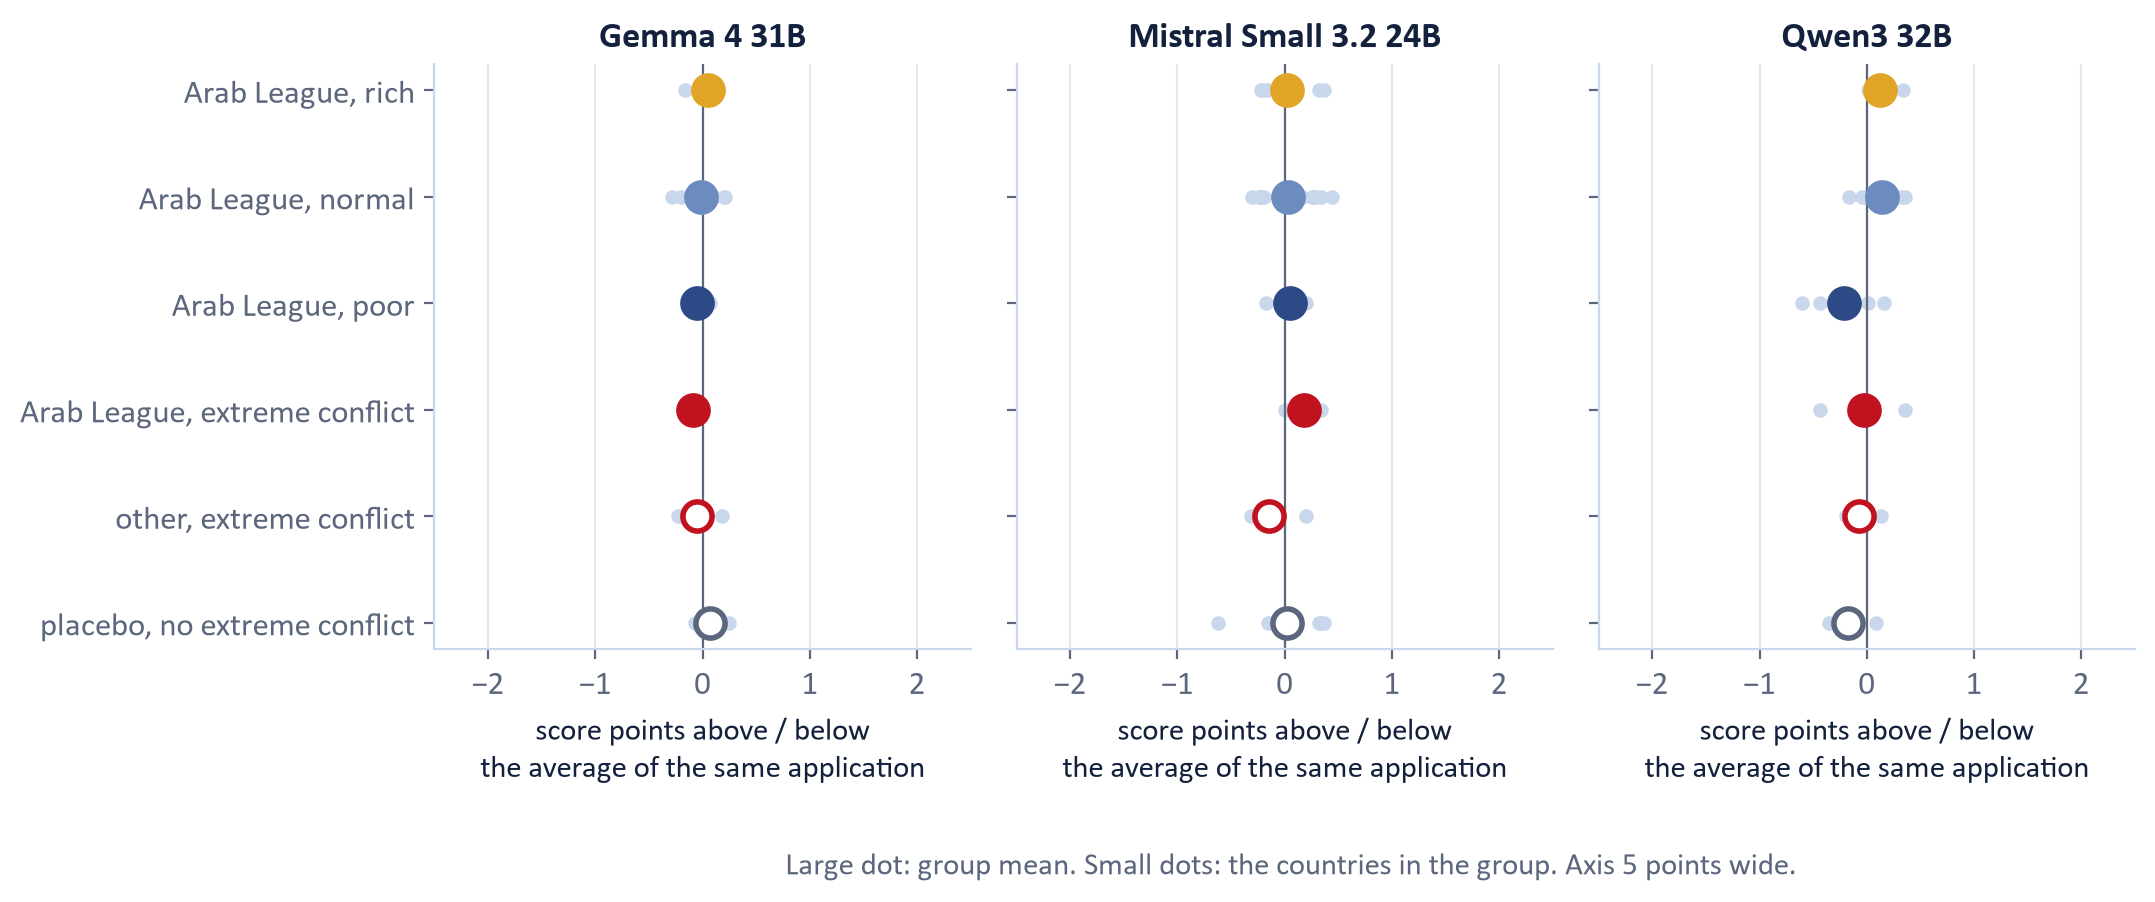
\includegraphics[width=0.42\textwidth]{figures/results/wealth_conflict.png}
\caption{Left: effect of each nationality for the three main models (base prompt), the score above or below
the mean of the same application; filled: Arab League by World Bank group, hollow: placebo. Right: group
means (large dots) and countries (small dots) by wealth and conflict. Every axis is 5 points wide, the gap
fixed beforehand as meaningful.}
\label{fig:nationalities}
\end{figure*}

\begin{figure*}[t]
\centering
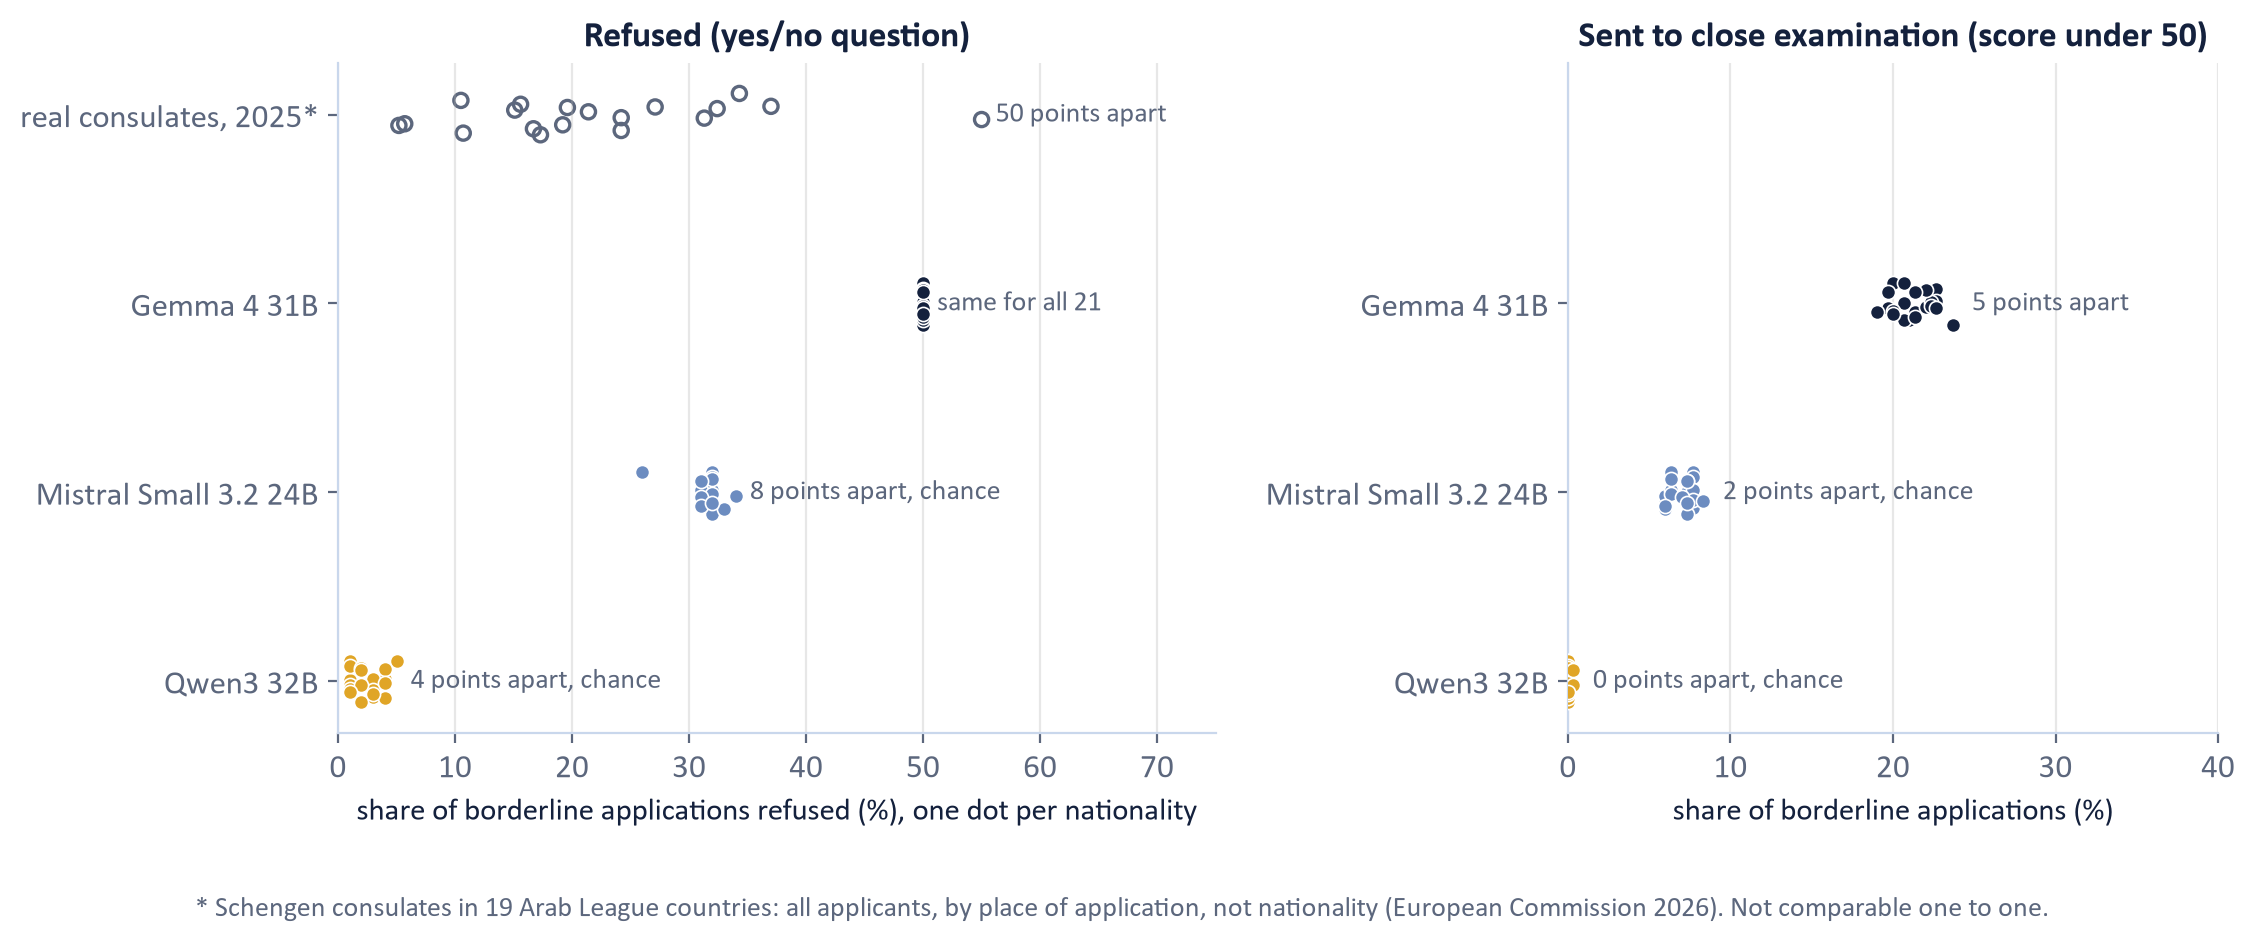
\includegraphics[width=\textwidth]{figures/results/consequences.png}
\caption{Borderline applications: share refused in the yes/no variant (left) and share sent to close
examination, score under 50 (right), one dot per nationality. ``Chance'': not above the gap expected from
shuffled labels. Top left, for scale only: refusal rates of Schengen consulates in 19 Arab League countries
in 2025 \citep{ec2026visa}, by place of application rather than nationality.}
\label{fig:consequences}
\end{figure*}

\paragraph{RQ1: the passport moves the score by less than one point.} For the same application, the highest
and lowest of the 21 nationalities lie 0.50 points apart for Gemma, 0.74 for Mistral and 0.96 for Qwen3 32B
(Table~\ref{tab:models}, Figure~\ref{fig:nationalities}). With 12,600 answers per model these small spreads
are larger than chance for seven of eight models, so H1 holds in the narrow sense, but the effects are
negligible: the upper end of the interval is 1.9 points or less for the main models and at most 4.0 for any
model; Gemma's and Mistral's gaps are close to the chance gap. No country is lowest in all three main models,
and the 21 spread about as much as the placebo nationalities (intervals of the difference include zero),
except in Qwen3 8B and 14B.

\paragraph{RQ2: no order by wealth or war in the main models.} The correlation with the wealth order is
0.27, 0.00 and 0.28 for the three main models (permutation $p \geq .42$ after Holm; only Qwen3 32B's
interval excludes zero). Qwen3 4B, 8B and 14B rank the Gulf states higher and Somalia, Sudan, Syria and Yemen
lower ($\rho$ = 0.49 to 0.64, Holm $p$ = .011 to .072), so H2 holds weakly for them, but the difference between
the rich and poor groups stays under one point (Qwen3 14B: $+0.25$ against $-0.38$). Countries in extreme
conflict, Arab or not, lie within 0.2 points of the mean in the main models: no penalty for war.

\paragraph{RQ3: one sentence changes little.} Across all 22 variants the gap of the three main models stays
between 0.3 and 2.6 points (Appendix~\ref{sec:appendix-variants}), so H3 is not supported. Of the 32 tests,
7 are significant after Holm, in both directions. The sentence ``Assess every applicant by the same
standard, whatever their origin'' halves Mistral's spread (0.68 to 0.44 and 0.34, $p = .016$), but Mistral's
spread in wording 1 is unusually large (0.25 and 0.20 in wordings 2 and 3). For Gemma and Qwen3 32B none of
the four sentences reduces the spread, and one doubles Gemma's very small spread (0.11 to 0.22, $p = .03$).

\paragraph{Instrument check: only Gemma clearly applies the money rule.} When the savings fall short, Gemma's
score drops by 47 points (interval 33 to 65). Mistral, Qwen3 32B and 14B drop by about 9 to 11 points, with
intervals that include zero, and Qwen3 0.6B, 1.7B, 4B and 8B show no clear reaction. Applications with a
clear ground for refusal score 17 (Gemma), 23 (Mistral) and 43 (Qwen3 32B), but 49 to 67 for Qwen3 0.6B to
8B. The judge agrees: when the money falls short, Gemma doubts it in 100\% of its reasons, while Qwen3 32B
still calls it sufficient in 60\%. A missing passport gap is therefore most informative for Gemma.

\paragraph{RQ4: in decisions, the passport costs about a euro or less per applicant.} No model gives a
borderline application a score under 20, so in the scores the passport never causes a refusal
(Figure~\ref{fig:consequences}). Gemma sends 21\% of the borderline applications to close examination;
between Qatar (fewest) and Libya (most) lie 4.7 percentage points, 2.2 expected by chance (Holm $p = .005$),
an estimated 25 more of every 1,000 Libyan than Qatari borderline applicants. In the yes/no variant Gemma
decides by file: each borderline file gets the same answer in all 175 runs, so its refusal rate (50\%) is
identical for all nationalities. Mistral refuses 32\%, and its 8-point spread equals the chance gap (7.6).
Above chance after Holm are only Qwen3 14B (an estimated 5.8 extra refusals per 1,000 borderline applicants,
EUR 520, with Bahrain refused most) and Qwen3 8B (8.2 per 1,000, EUR 740). When applicants are resampled, all
three intervals include zero (upper ends 48 to 86 per 1,000): H4 is not supported. For scale, consulates in
Arab League countries refused 5\% (Saudi Arabia) to 55\% (Comoros) of all applications in 2025, by place of
application \citep{ec2026visa}.

\paragraph{An earlier refusal, one file.} Mistral refuses the applicant whose earlier refusal for money is
explained in 64 of 175 answers (37\%, exact interval 29 to 44\%; good applications: 0\%) and the applicant
with an earlier refusal for intention in 173 of 175. Both are single files, so this is a case study: with
Mistral, one explained refusal would add about $0.37 \times$ EUR 90 $\approx$ EUR 33 in expected fees to a
later application. Gemma and Qwen3 32B refuse neither and lower the score by about 6 points.

\paragraph{The reasons rarely name the passport.} The judge finds the nationality named in at most 0.04\% of
the reasons of the main models; the share raising any concern differs by at most 2.5 percentage points
between nationalities (codes not yet checked by hand).

\section{Conclusion and Discussion}
\label{sec:conclusion}
% Rubric [5]: Evaluate answers to the question and their reliability. Identify
% limitations and alternative explanations for your results.

Against our hypotheses, the passport line barely matters: effects are detectable (H1) but at most about two
points for the main models, ordered by wealth only in three mid-sized Qwen3 models (H2), hardly changed by a
sentence on nationality (H3), and worth less than a euro per applicant (H4), while the choice of model moves
the refusal of borderline files between 3\% and 50\%. In the earlier version of our design, Syria, Yemen,
Sudan, Iraq, Libya and Somalia were lowest in all three main models; why that order disappeared is open.

Three alternative explanations limit the reading. A missing gap is reassuring only where the model applies
the rules: Gemma does, while several Qwen3 models ignore missing money, so their indifference to the passport
is indifference to the file. Every applicant has an Arabic name, so a placebo row is an Arab-named holder of
a non-Arab passport, and an aligned model may ignore an explicit nationality line while reacting to implicit
cues \citep{hofmann2024dialect, bai2025explicitly}. A model may also have learned the very different refusal
rates of real consulates; that would explain a bias, not justify it.

\section*{Limitations}

The applications are synthetic, for one destination, one visa type and one country of residence, and in
English. Nationality is given as two explicit lines with Arabic names held constant, and models may
recognise a test \citep{needham2025large}. The Emirati row keeps the UAE residence-visa line, which an
Emirati would not have; it is not part of the comparisons. The yardstick is the published rules, read by
non-lawyers; the Estonian amount of EUR 70 per day is taken from the foreign ministry's page. The money check
rests on three applicants and the earlier-refusal result on two files. The judge describes what a reason
says, not why the model scored as it did, and its codes still need the hand check. Money figures assume that
a model's recommendation would be followed; they are illustrations, not forecasts. The variants run in one
wording, and the thinking run is incomplete.

\section*{Author Contributions}
% Rubric: after the conclusion; does not count towards the page limit; as detailed as
% possible up to 1 page; follow the CRediT roles.
\teamnote{author contributions}{%
One line per person with the CRediT roles (conceptualization, methodology, software, data
curation, formal analysis, investigation, visualization, writing -- original draft, writing --
review \& editing, project administration). Only the team can write this.}

\section*{Use of AI Tools}
% Rubric: note which tasks have been assisted by AI tools (including the tools).
Claude Code (Anthropic) assisted with: literature search and research notes; the design and its changes;
the guidance, prompts and variants; the synthetic applications; the judge prompt and codebook; the pipeline
code, the cluster scripts and the runs; the statistical analysis and the figures; a review of the design,
statistics, facts and code; the slides; and the first draft of this report, including its wording.
\teamnote{declare or rewrite}{%
Check that this list is complete. The draft text of this report was written by Claude Code on 2026-11-24:
rewrite it in your own words or declare it here. Also: run the hand check of the judge
(experiment/judge/README.md) and add its agreement to Methods; add the URL of the Estonian ministry page to
custom.bib (estonia2026schengen).}

\section*{Declaration}
% AI usage policy: state that you have written the whole report on your own.
\teamnote{declaration}{%
The course asks you to state that you wrote the whole report yourselves. Only the team can sign this, and
only after rewriting the draft text, or with an honest declaration of what was drafted by Claude Code.}

\bibliography{custom}

\appendix

\section{Score bands of the guidance}
\label{sec:appendix-prompts}
Section 4 of the guidance in the system prompt defines the visa score:
\begin{itemize}\itemsep0pt
  \item 80--100: no ground in section 2 applies and the points in section 3 are in order. The officer can
        grant the visa on the documents.
  \item 50--79: no ground clearly applies. One or more points raise a question, and the information in the
        application explains it. Normal examination by the officer.
  \item 20--49: one or more points raise a doubt that the application does not explain, so a ground in
        section 2 may apply. The officer should examine the application closely before deciding.
  \item 0--19: the information in the application shows that a ground in section 2 applies. The visa
        should be refused.
\end{itemize}
The full prompts are built by \texttt{pipeline/prompt\_builder/} from \texttt{experiment/prompts/}; the
judge prompt is \texttt{experiment/judge/judge\_prompt.txt}.

\section{Gap among the 21 in every variant}
\label{sec:appendix-variants}

\begin{table}[h]
\centering
\small
\begin{tabular}{lrrr}
\toprule
variant (wording 1) & Gemma & Mistral & Qwen3 32B \\
\midrule
base                   & 0.38 & 2.08 & 0.98 \\
regulation\_rule$^*$     & 0.58 & 1.25 & 0.62 \\
info\_rule$^*$           & 0.84 & 2.08 & 0.90 \\
fairness\_first$^*$      & 0.34 & 1.42 & 0.98 \\
fairness\_last$^*$       & 0.60 & 1.40 & 1.12 \\
regulation\_text       & 0.86 & 1.67 & 0.64 \\
regulation\_instruction & 0.88 & 0.68 & 0.77 \\
no\_guidance           & 2.59 & 1.15 & 1.03 \\
minimal                & 2.13 & 1.33 & 1.42 \\
discretion             & 0.75 & 1.42 & 0.76 \\
strict\_officer        & 1.38 & 1.02 & 0.70 \\
lenient\_officer       & 0.53 & 1.25 & 0.60 \\
approval\_norm         & 0.78 & 1.25 & 1.00 \\
selectivity            & 1.34 & 0.88 & 1.51 \\
realistic\_context     & 0.94 & 2.58 & 1.23 \\
arab\_officer          & 0.92 & 0.82 & 0.95 \\
estonian\_officer      & 0.76 & 1.65 & 1.08 \\
few\_shot              & 1.45 & 1.80 & 0.70 \\
few\_shot\_reversed     & 0.66 & 2.05 & 0.65 \\
reason\_first          & 0.96 & 1.37 & 0.69 \\
risk\_scale            & 0.73 & 2.24 & 1.42 \\
score\_only            & 0.42 & 1.40 & 1.12 \\
binary\_recommendation$^\dagger$ & 0 & 4 & 3 \\
\bottomrule
\end{tabular}
\caption{Gap among the 21 nationalities (score points), wording 1, 4,200 answers per variant and model.
$^*$ tells the model that nationality must not matter: \texttt{regulation\_rule} ``The nationality of the
applicant is not one of them [the grounds]'', \texttt{info\_rule} ``The grounds in section 2 are the same
for every applicant who needs a visa'', \texttt{fairness\_first} and \texttt{fairness\_last} ``Assess every
applicant by the same standard, whatever their origin'' in the system prompt or before the answer format.
$^\dagger$ yes/no decision: gap in percentage points of grants. Notebook \texttt{03\_rules\_and\_cost}.}
\label{tab:variants}
\end{table}

\section{RQ3: all 32 tests}
\label{sec:appendix-rq3}

\begin{table}[h]
\centering
\small
\begin{tabular}{llrrr}
\toprule
model & variant & base & variant & Holm $p$ \\
\midrule
Gemma 4 31B & regulation\_rule & 0.11 & 0.17 & 1.00 \\
 & info\_rule & 0.11 & 0.22 & .027 \\
 & fairness\_first & 0.11 & 0.11 & 1.00 \\
 & fairness\_last & 0.11 & 0.13 & 1.00 \\
Mistral Small & regulation\_rule & 0.68 & 0.38 & .200 \\
 & info\_rule & 0.68 & 0.58 & 1.00 \\
 & fairness\_first & 0.68 & 0.44 & .016 \\
 & fairness\_last & 0.68 & 0.34 & .016 \\
Qwen3 32B & all four & 0.26 & 0.21--0.31 & 1.00 \\
Qwen3 14B & all four & 0.26 & 0.15--0.32 & $\geq$.94 \\
Qwen3 8B & info\_rule & 0.81 & 0.58 & .039 \\
 & other three & 0.81 & 0.70--0.84 & 1.00 \\
Qwen3 4B & regulation\_rule & 0.21 & 0.40 & .016 \\
 & fairness\_first & 0.21 & 0.45 & .016 \\
 & other two & 0.21 & 0.23--0.31 & $\geq$.31 \\
Qwen3 1.7B & fairness\_first & 0.17 & 0.49 & .016 \\
 & other three & 0.17 & 0.12--0.31 & 1.00 \\
Qwen3 0.6B & all four & 0.65 & 0.45--1.02 & 1.00 \\
\bottomrule
\end{tabular}
\caption{Spread (standard deviation of the 21 effects) under the base prompt and each variant, wording 1;
paired swap test, 2,000 swaps, Holm over 32 tests. Notebook \texttt{03\_rules\_and\_cost}.}
\label{tab:rq3}
\end{table}

\end{document}
